\begin{activity} \label{A:2.8.2}  
The following prompts in this activity will lead you to develop the derivative of the inverse tangent function.
\ba
	\item Let $r(x) = \arctan(x)$.  Use the relationship between the arctangent and tangent functions to rewrite this equation using only the tangent function.
	\item Differentiate both sides of the equation you found in (a).  Solve the resulting equation for $r'(x)$, writing $r'(x)$ as simply as possible in terms of a trigonometric function evaluated at $r(x)$.
	\item Recall that $r(x) = \arctan(x)$.  Update your expression for $r'(x)$ so that it only involves trigonometric functions and the independent variable $x$.
	\item Introduce a right triangle with angle $\theta$ so that $\theta = \arctan(x)$.  What are the three sides of the triangle?
	\item In terms of only $x$ and $1$, what is the value of $\cos(\arctan(x))$?
	\item Use the results of your work above to find an expression involving only $1$ and $x$ for $r'(x)$.
\ea
\end{activity}
\begin{smallhint}
\ba
	\item Recall that for any function and its inverse, writing $y = f^{-1}(x)$ is equivalent to writing $f(y) = x$.
	\item Apply the chain rule to differentiate $\tan(r(x))$.
	\item This question is only asking you to substitute the expression for $r(x)$ into what you found in (b).
	\item Let the vertical leg of the triangle be $x$.  What must the horizontal leg be?
	\item Recall that the cosine of an angle is the length of the adjacent leg over the length of they hypotenuse.
	\item Note that $\cos^2(\alpha) = (\cos(\alpha))^2.$
\ea
\end{smallhint}
\begin{bighint}
\ba
	\item Recall that for any function and its inverse, writing $y = f^{-1}(x)$ is equivalent to writing $f(y) = x$.
	\item Remember that $\frac{d}{dx}[\tan(u(x))] = \sec^2(u(x)) u'(x)$.
	\item This question is only asking you to substitute the expression for $r(x)$ into what you found in (b).
	\item Let the vertical leg of the triangle be $x$.  What must the horizontal leg be?  From there, how can you find the hypotenuse?
	\item Recall that the cosine of an angle is the length of the adjacent leg over the length of they hypotenuse.
	\item Note that $\cos^2(\alpha) = (\cos(\alpha))^2.$
\ea\end{bighint}
\begin{activitySolution}
\ba
	\item Since $r(x) = \arctan(x)$, it is equivalent to write $\tan(r(x)) = x$.
	\item Differentiating, we have $\frac{d}{dx}[\tan(r(x))] = \frac{d}{dx}[x]$, so
	$$\sec^2(r(x)) r'(x) = 1,$$
	and thus 
	$$r'(x) = \frac{1}{\sec^2(r(x))} = \cos^2(r(x)),$$
	since $\frac{1}{\sec(\alpha)} = \cos(\alpha).$
	\item Since $r(x) = \arctan(x)$, we now have that $r'(x) = \cos^2(\arctan(x)).$
	\item Letting $\theta = \arctan(x)$, it follows that we can view $\theta$ as an angle in a right triangle with legs $1$ and $x$ (so that $\tan(\theta) = \frac{x}{1}$, and thus by the Pythagorean Theorem, the triangle's hypotenuse is $\sqrt{1+x^2}$, as shown below.
	\begin{center}
	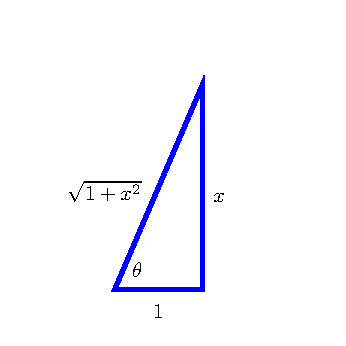
\includegraphics{figures/2_6_cosarctan.eps}
	\end{center}
	\item To evaluate $\cos(\arctan(x))$, we use the right triangle developed in (d) and observe that 
	$$\cos(\arctan(x)) = \frac{1}{\sqrt{1+x^2}}.$$
	\item Finally, we recall that we know $r'(x) = \cos^2(\arctan(x)) = \left( \cos(\arctan(x)) \right)^2$.  Having established that $\cos(\arctan(x)) = \frac{1}{\sqrt{1+x^2}}$, we now have that
	$$r'(x) = \frac{1}{1+x^2}.$$
\ea
\end{activitySolution}
\aftera